\subsubsection{\stid{6.02} LLNL ATDM Math Libraries}

\paragraph{Overview}

The LLNL ATDM Mathematical Libraries project performs work in the MFEM library
\cite{MFEM} that is focused on providing high-performance mathematical algorithms
and finite element discretizations to next-gen high-order ECP/ATDM
applications. A main component of these efforts is the development of
ATDM-specific physics enhancements in the finite element algorithms in MFEM and
the MFEM-based BLAST Arbitrary Lagrangian-Eulerian (ALE) code \cite{BLAST}, in
order to provide efficient discretization components for LLNL's ATDM efforts,
including the MARBL application (ECP's LLNLApp).

A second main task in the project is the development of unique unstructured
adaptive mesh refinement (AMR) algorithms in MFEM, that focus on generality,
parallel scalability, and ease of integration in unstructured mesh
applications. The new AMR capabilities can benefit a variety of ECP apps that
use unstructured meshes, as well as many other applications in industry and the
SciDAC program.

Another aspect of the work is the preparation of the MFEM finite element library
and related codes for exascale platforms by using mathematical algorithms and
software implementations that exploit increasing on-node concurrency targeting
multiple complex architectures (e.g. GPUs). This part of the project is
synergistic with and leverages efforts from the ECP CEED co-design center.

MFEM is an open-source finite element library with ~3000 downloads/year from 70+
countries. It is freely available at \url{mfem.org}, on GitHub
at \url{github.com/mfem}, where the MFEM community includes more than 165
members), as well as via Spack and OpenHPC. The application outreach and the
integration in the ECP ecosystem is further facilitated by MFEM's participation
in ECP's xSDK project.

\paragraph{Key Challenges}

The key challenges addressed by the LLNL ATDM Mathematical Libraries project are:

\noindent
{\bf \em Robust high-order finite element methods for ALE compressible flow.}
While high-order methods offer significant advantages in terms of HPC performance,
their application to complicated ALE problems requires careful considerations to
control oscillations and ensure accuracy.

\begin{figure}[htb]
\centering
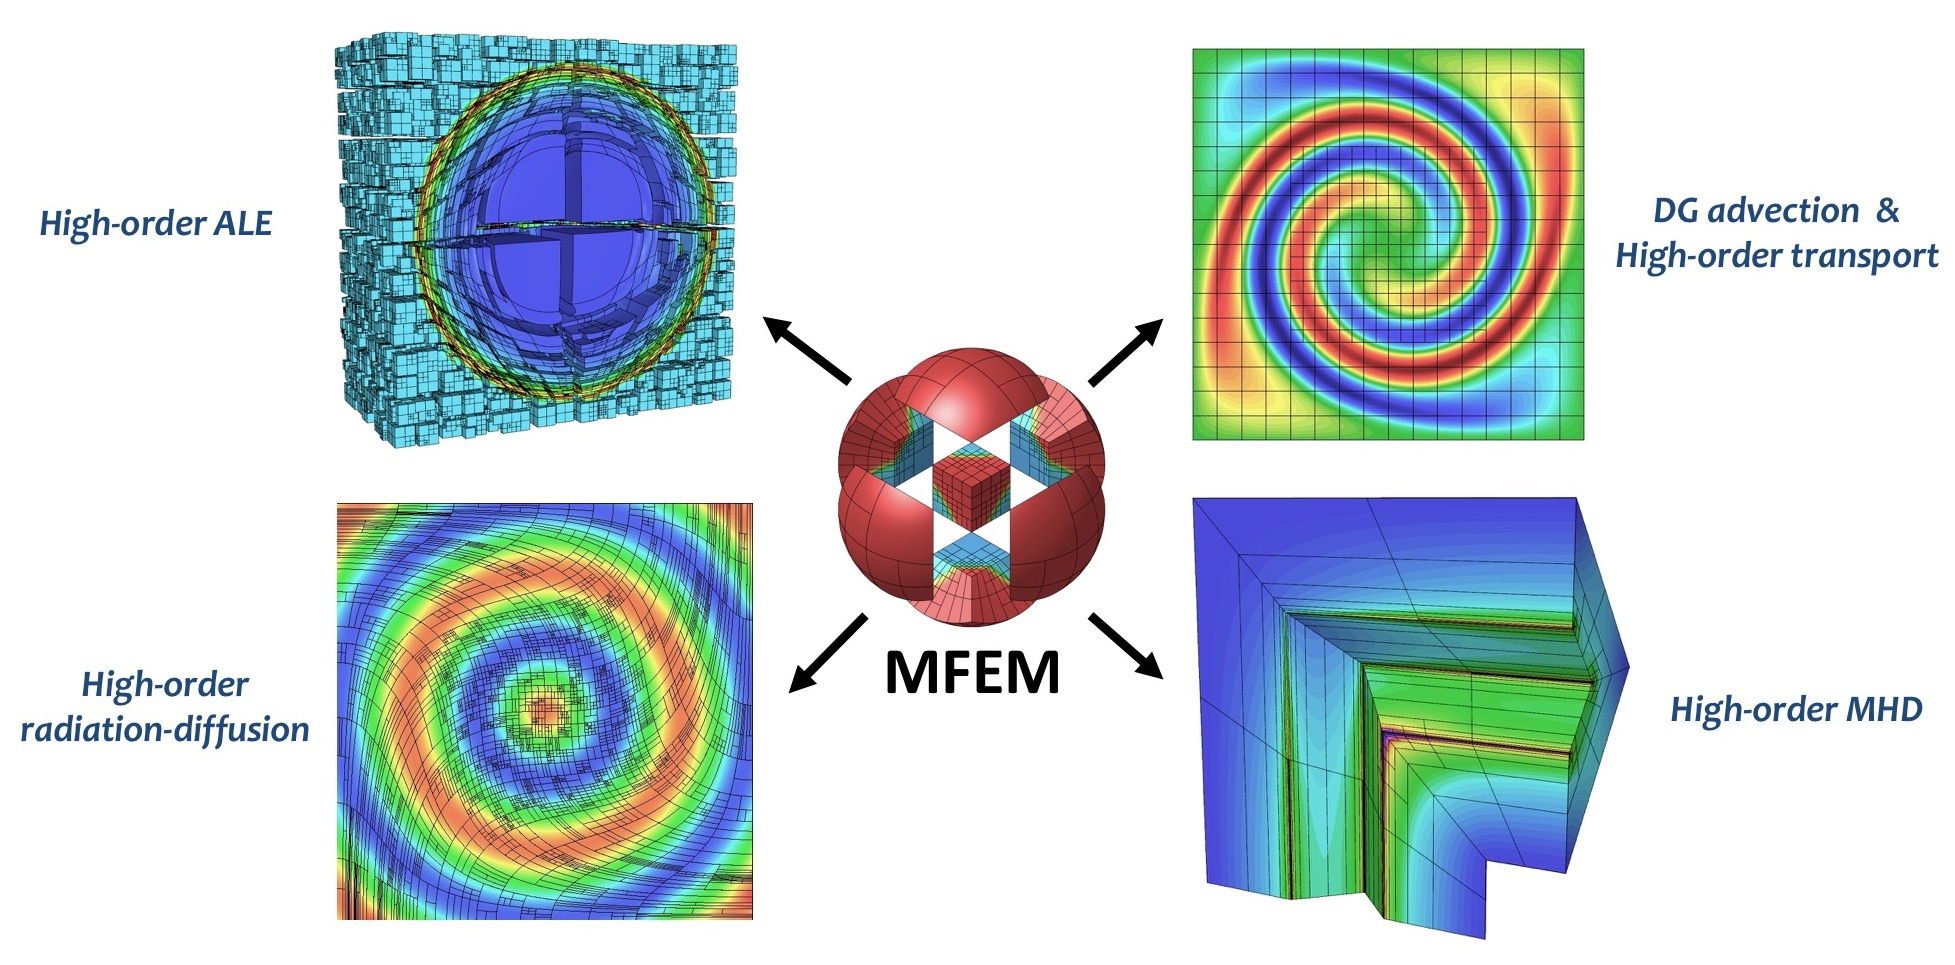
\includegraphics[width=\textwidth]{projects/2.3.6-NNSA/2.3.6.02-LLNL-ATDM/mfem-amr}
\caption{\label{fig:mfem-amr}AMR implementation in MFEM allows many applications to benefit from non-conforming adaptivity, without significant changes in their codes.}
\end{figure}

\noindent
{\bf \em Scalable algorithms for unstructured adaptive mesh refinement.}
Adaptive mesh refinement is a common way to increasing application efficiency
in problems with localized features. While block-structured AMR has been
well-studied, applying AMR in unstructured settings is challenging, especially
in terms of derefinement, anisotropic refinement, parallel rebalance and
scalability.

\noindent
{\bf \em GPU porting of finite element codes.}
Due to the relatively high complexity of the finite element machinery, MFEM,
BLAST and related codes use object-oriented C++ design that allows generality
and flexibility, but poses challenges in terms of porting to GPU architectures.
Finding the right balance between generality and performance in the GPU context
is an important challenge for many finite element-based codes that remains
outstanding in the current software and programming model environment.

\paragraph{Solution Strategy}

The MFEM team has performed and documented a lot of research in
high-performance mathematical algorithms and finite element discretizations
of interest to ATDM applications
\cite{BLAST18,BLASTFCT18,BLASTFCT17,BLAST16,BLAST14,BLAST13,BLAST12,BLAST11}.
Our work has demonstrated that the high-order finite element approach can
successfully handle coupled multi-material ALE, radiation-diffusion and MHD.
We have also shown how high-order methods can be adapted for monotonicity
(positivity preservation), handling of artificial viscosity (shock capturing),
sub-zonal physics via closure models, etc.

To enable many applications to take advantage of unstructured mesh adaptivity,
the MFEM team is developing AMR algorithms at library level, targeting both
{\em conforming} local refinement on simplex meshes and {\em non-conforming}
refinement for quad/hex meshes. Our approach is fairly general, allowing for
any high-order finite element space, H1, H(curl), H(div), on any high-order
curved mesh in 2D and 3D, arbitrary order hanging nodes, anisotropic refinement,
derifenement and parallel load balancing.
An important feature of our library approach is that it is independent of
the physics, and thus easy to incorporate in apps, see Figure \ref{fig:mfem-amr}.

As part of the efforts in the ECP co-design Center for Efficient Exascale
Discretizations (CEED), the MFEM team is also developing mathematical algorithms
and software implementations for finite element methods that exploit increasingq
on-node concurrency targeting multiple complex architectures (e.g. GPUs). This
work includes the libCEED low-level API library, the Laghos miniapp, and several
other efforts available through CEED.

To reach its many customers and partners in NNSA, DOE Office of Science, academia
and industry, the MFEM team delivers regular releases on GitHub (e.g. mfem-3.3 and
mfem-3.3.2 in 2017, mfem-3.4 in 2018) that include detailed documentation and
many example codes.
Code quality is ensured by smoke tests with Travis CI on Linux, Mac, Windows and
nightly regression testing at LLNL.

\paragraph{Recent Progress}

Selected recent highlights:
\begin{itemize}
\item
Developed a new formulation for discretizing problems with 1D spherical symmetry
in BLAST. Extended BLAST to the 3T-model (separate equations for the electron
and ion internal energies). Added support for changing masses during the
Lagrangian phase.
\item
Completed the delivery of discretization support for the FY18 MARBL ATDM L2
milestone, including new 3T radiation-diffusion algorithms, and a simulation
capability for problems with spherical and cylindrical symmetry via weight
adjustments. With this and other support from the MFEM team, the MARBL team
successfully defended its ATDM L2 milestone.
\item
Worked on high-order ALE algorithms in BLAST: developed remap step for density
component masses, various code improvements and bugs fixes related to L2
milestone.
\item
MFEM version 3.4 was released with many new features including: significantly
improved non-conforming unstructured AMR scalability; integration with PUMI;
block nonlinear operators and variable order NURBS; Conduit mesh blueprint
support; general high-order-to-low-order refined field transfer; new specialized
time integrators and 12 new examples and miniapps.
\item
Implemented an initial draft of MFEM’s ``engine'' interface extension to support
GPUs and other accelerators. Performed tests with the new ``engine'' extension
on Sierra. Explored its use in the Laghos miniapp and BLAST.
\item
Improvements in AMR interpolation matrix for better construction of
communication groups and performance monitoring in the Laghos miniapp.
\item
Several AMR improvements, including better local conforming tetrahedral
refinement (collaborating with a GitHub user), fix for boundary coefficient
projection, and general communication groups on for non-conforming AMR
supporting the AMR integration in BLAST.
\item
With summer student made progress on matrix-free algorithms for high-order field
monotonicity, targeting performance improvements in the remap phase of
MARBL/BLAST.
\item
GLVis version 3.4 was released with several new features including: 10 new color
palettes, better multi-screen window manager support, capability to show element
and vertex numbering in 2D, use of X.509 certificates in secure sockets, and a
new CMake build system.
\item
Developed a new version of the hogtess high order experimental visualization
tool based on modern OpenGL 4.3 compute shaders that does correct cutting of
high order meshes in 3D.
\end{itemize}

\paragraph{Next Steps}

Our next steps include:
test the new engine API on Sierra using MFEM examples and the Laghos miniapp;
prepare and release the next version of MFEM, v4.0, with initial support for
GPU architectures;
continue to attend and contribute to the weekly MARBL and BLAST meetings;
and provide support for the upcoming MARBL L2 milestones.

